\documentclass[10pt,a4paper]{article}
\usepackage[utf8]{inputenc}
\usepackage{amsmath}
\usepackage{amsfonts}
\usepackage{amssymb}
\usepackage{tikz}
\usepackage{graphicx}
\author{James Lee}
\title{3rd Assignment of Computational Physics}
\begin{document}
	\maketitle
	\begin{abstract}
		In this report I present to you the a program that can print English using strings.
	\end{abstract}
	\section{Main Content}
	\subsection{Print a Name}
	The L1 program is able to print my name:
	\begin{figure}[htbp]
		\centering
		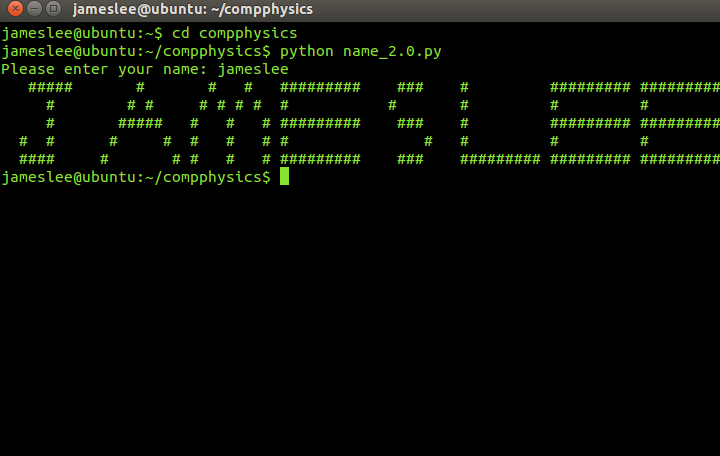
\includegraphics[width=5in]{name_1.png}
		\caption{Print Jameslee}
	\end{figure}
	\subsection{Print any Consequence of Letters}
	The L1 program is able to print any name:
	\begin{figure}[htbp]
		\centering
		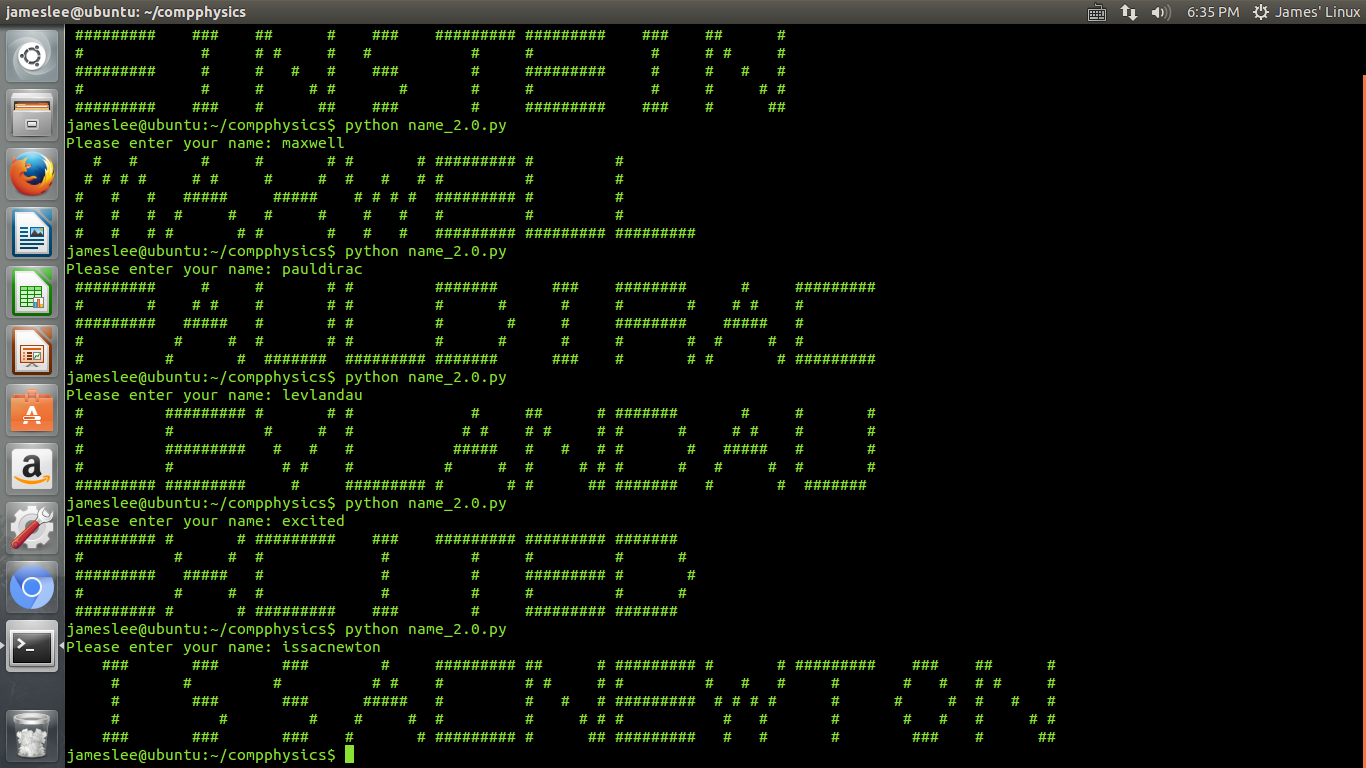
\includegraphics[width=7in]{name_2.png}
		\caption{Print Any Name}
	\end{figure}
	
	
    \section*{Acknowledgement}
    When tackling this assignment, I benefitted a lot from the valuable discussions with Liu Xingchen. I would like to thank him for pointing out several grammar errors I made, also, for his willingness to discuss with me.
    
    \begin{thebibliography}{99}
    	\bibitem{}Hunter J, the Matplotlib Documentation, 2016
    	\bibitem{}Giordano N.J, Nakanishi H, Computational Physics, Pearson Education, 2007
    \end{thebibliography} 
\end{document}